\chapter{ODE Example Revisited}\label{ext:ode-example}
One way by which modelers can improve the quality of parameter estimates is by collecting more data.
We consider what would happen if our measurement equipment were able to capture twice as many observations.
Furthermore, we verify computationally that using more precise measurement equipment improves the precision of the MUD estimate.

%%%%%%%%%%%%%%%%%%%%%%%%%%%%%%%%%%%%%%%%%%%%%%%%%%%%%%%%%%%%%%%%%%%%
\section{Different Measurement Equipment}
Instead of using equipment that operates at $100$Hz, we take $200$ measurements every second, resulting in 400 equispaced observations for $t \in (1,3)$.
All other choices involved in the experiment (assumed equipment tolerance, number of trials, parameter samples), are kept the same.
We refer to this setup wit faster measurement equipment as the ``alternative'' design.


We show the resulting predictions for the signal using MUD points from twenty repeated trials in Figure~\ref{fig:ode-alt-reference} using the first twenty (middle) and all of the measurements (bottom).
The top of the figure shows the solution from the original setup \ref{fig:ode-reference} for visual comparison.
The true signal is well-recovered even with a small subset of the data collected.
By the time all measurements are used, the stability of the solutions\---with respect to the noise that may have polluted them\---is evidenced by the fact that the red lines representing solutions disappear against the backdrop of the true signal in black.

\begin{figure}[htbp]
  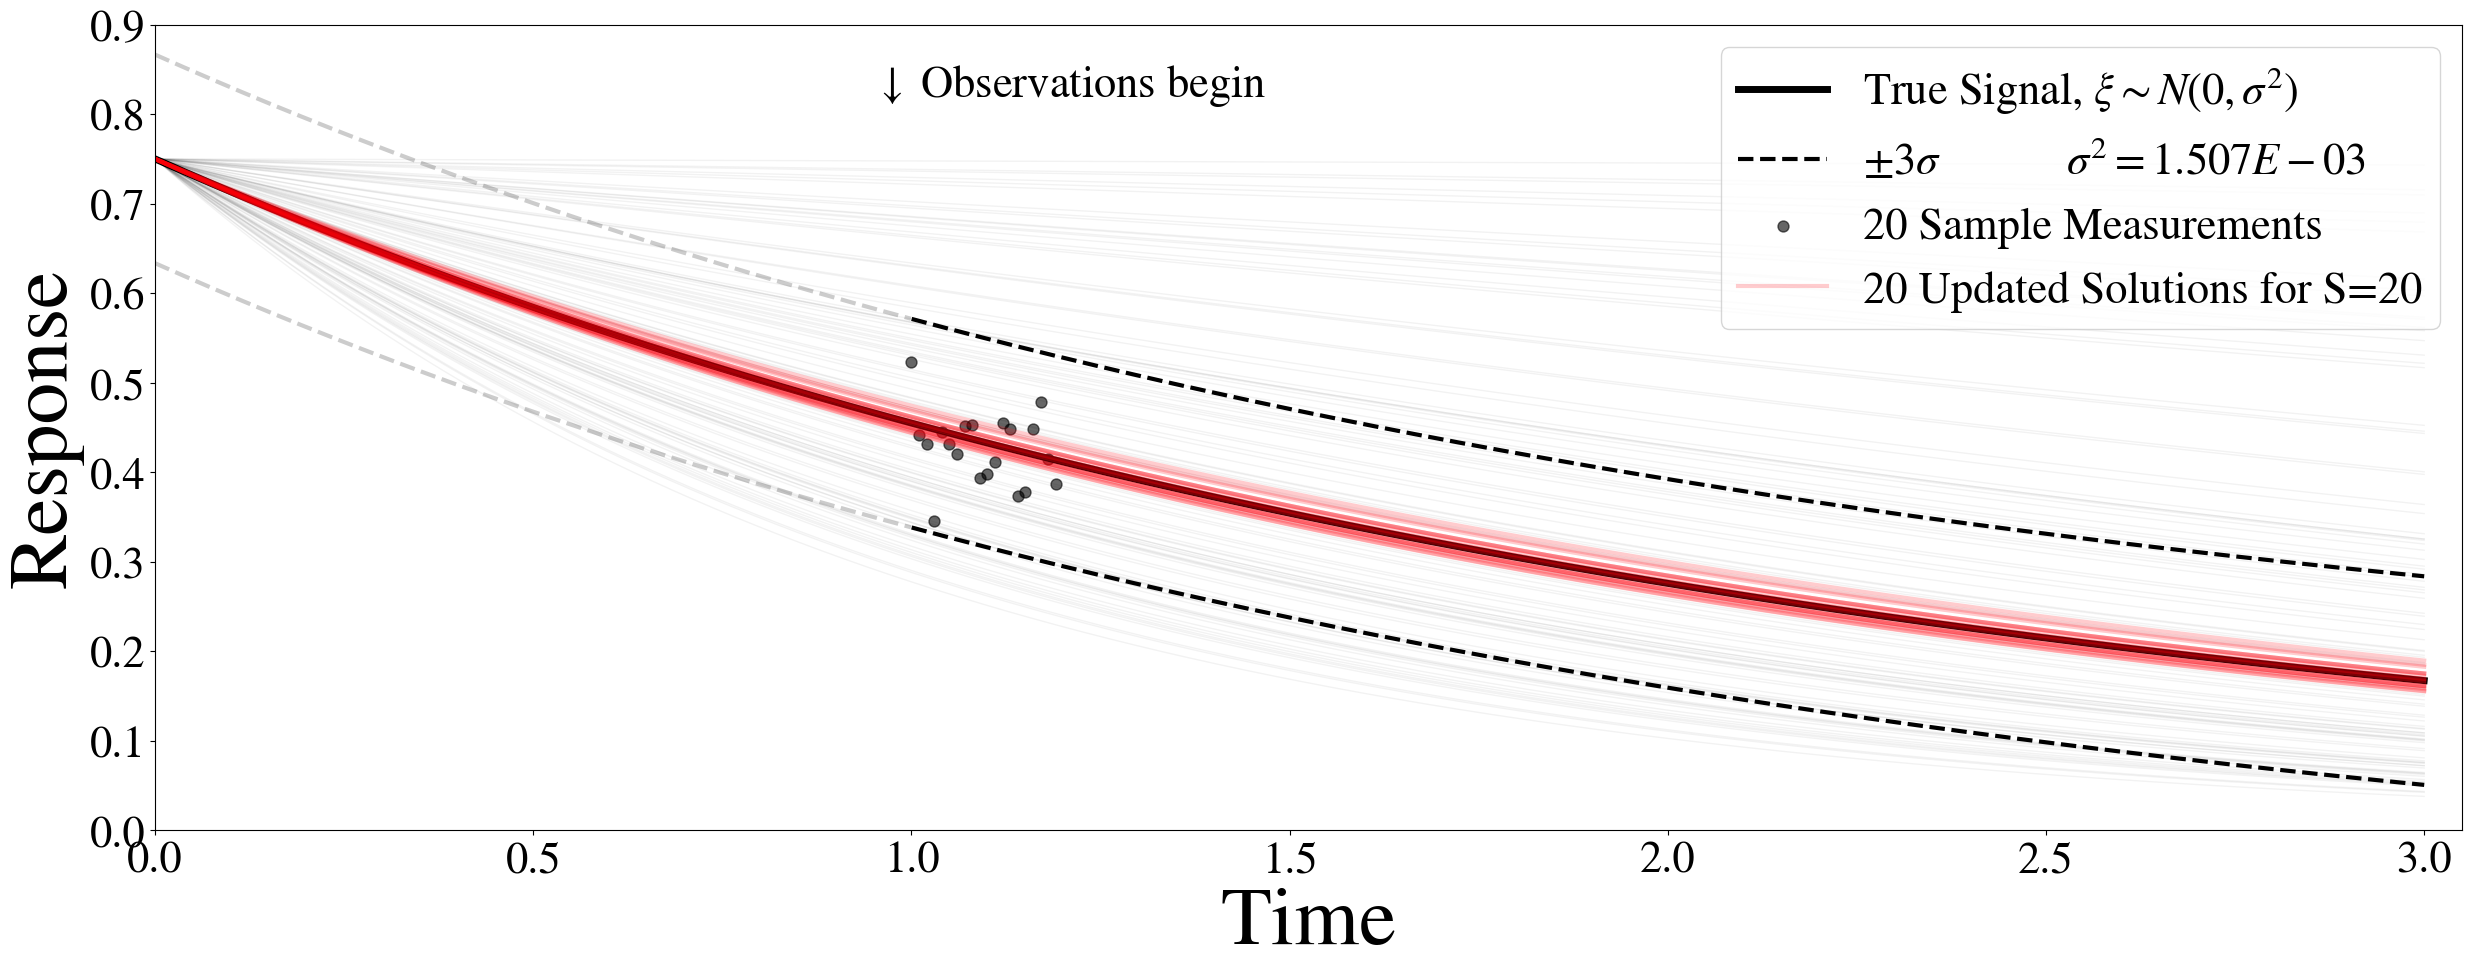
\includegraphics[width=\linewidth]{figures/ode/ode_20_reference_solution.png}
  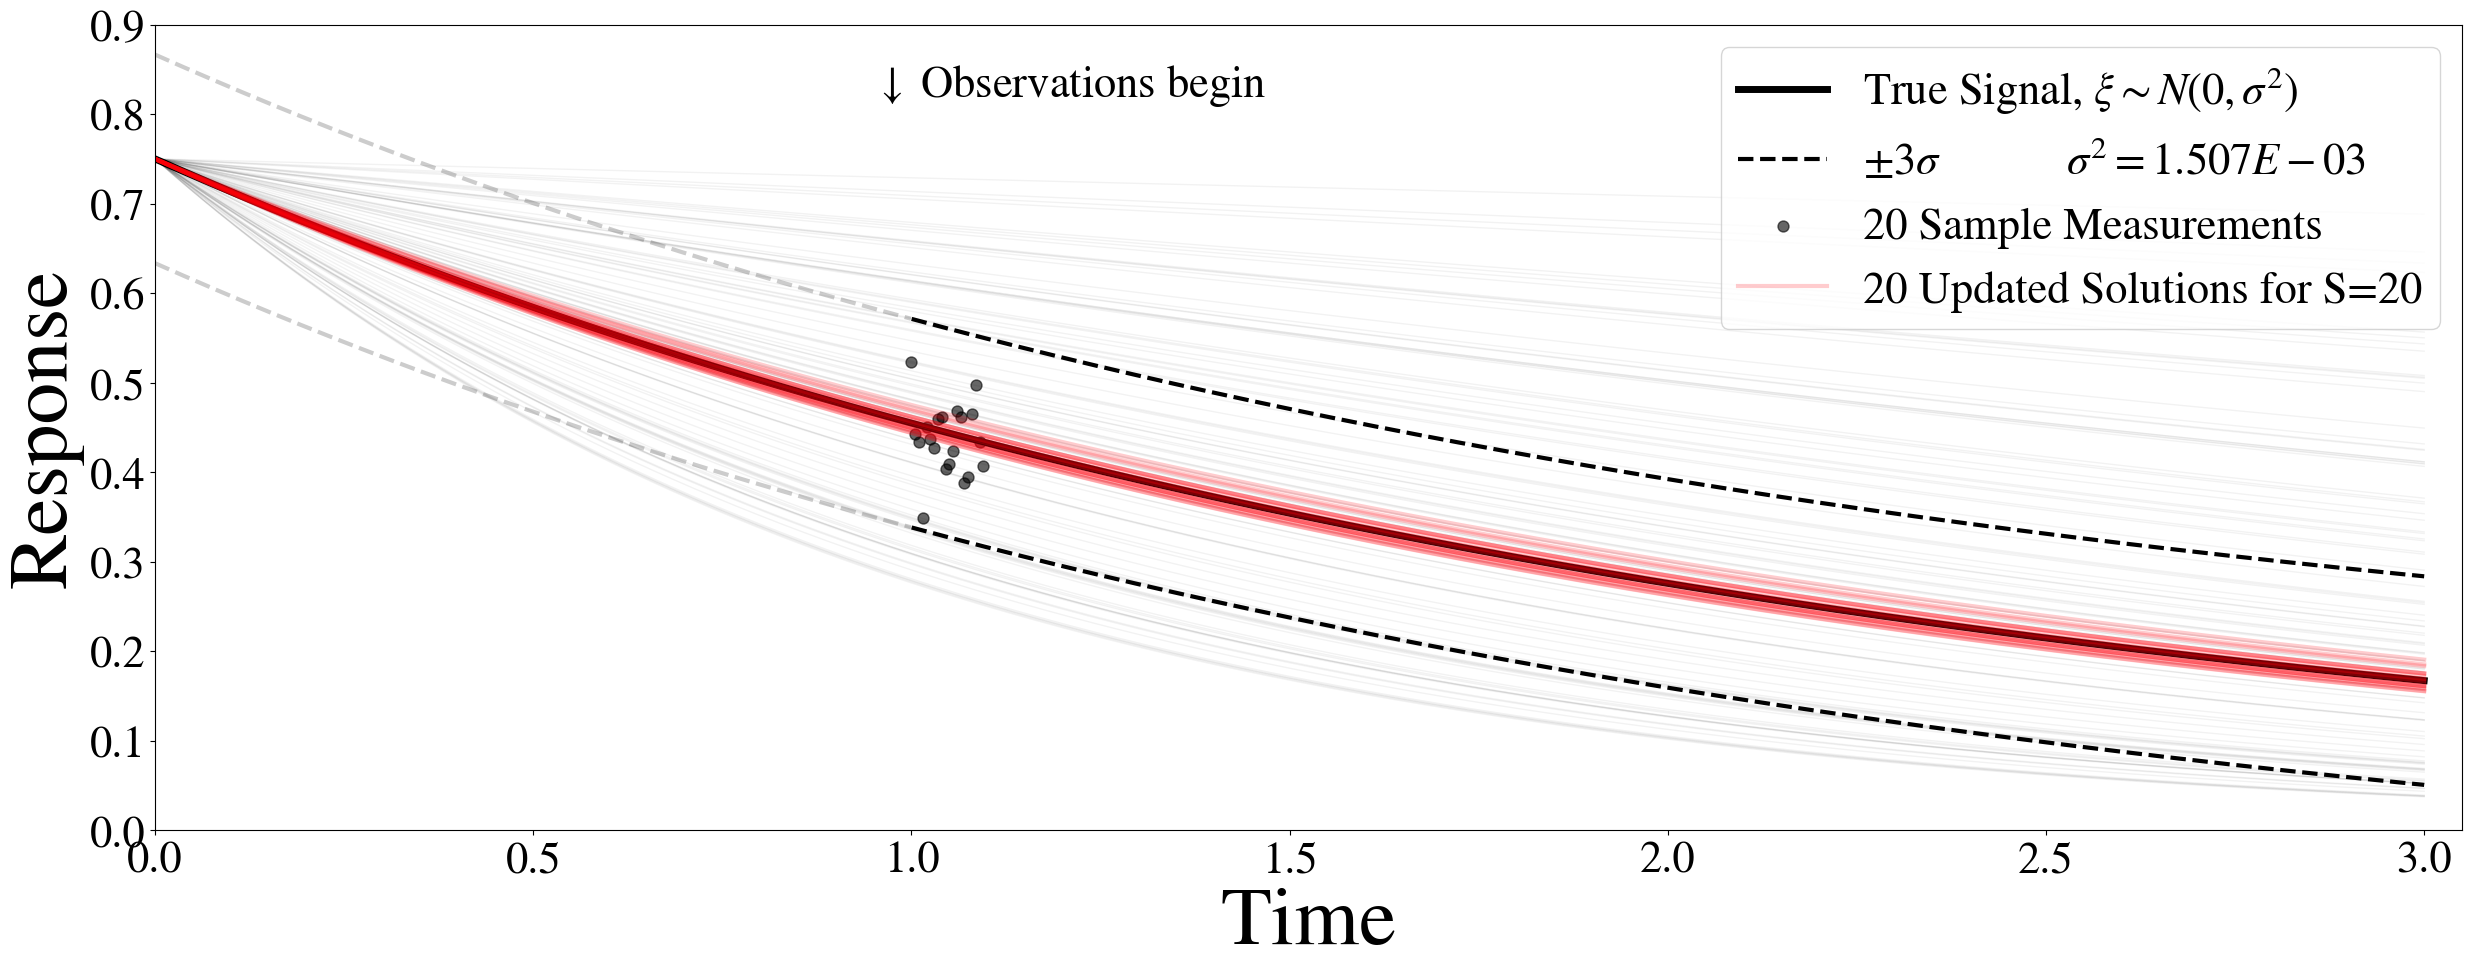
\includegraphics[width=\linewidth]{figures/ode/ode-alt_20_reference_solution.png}
  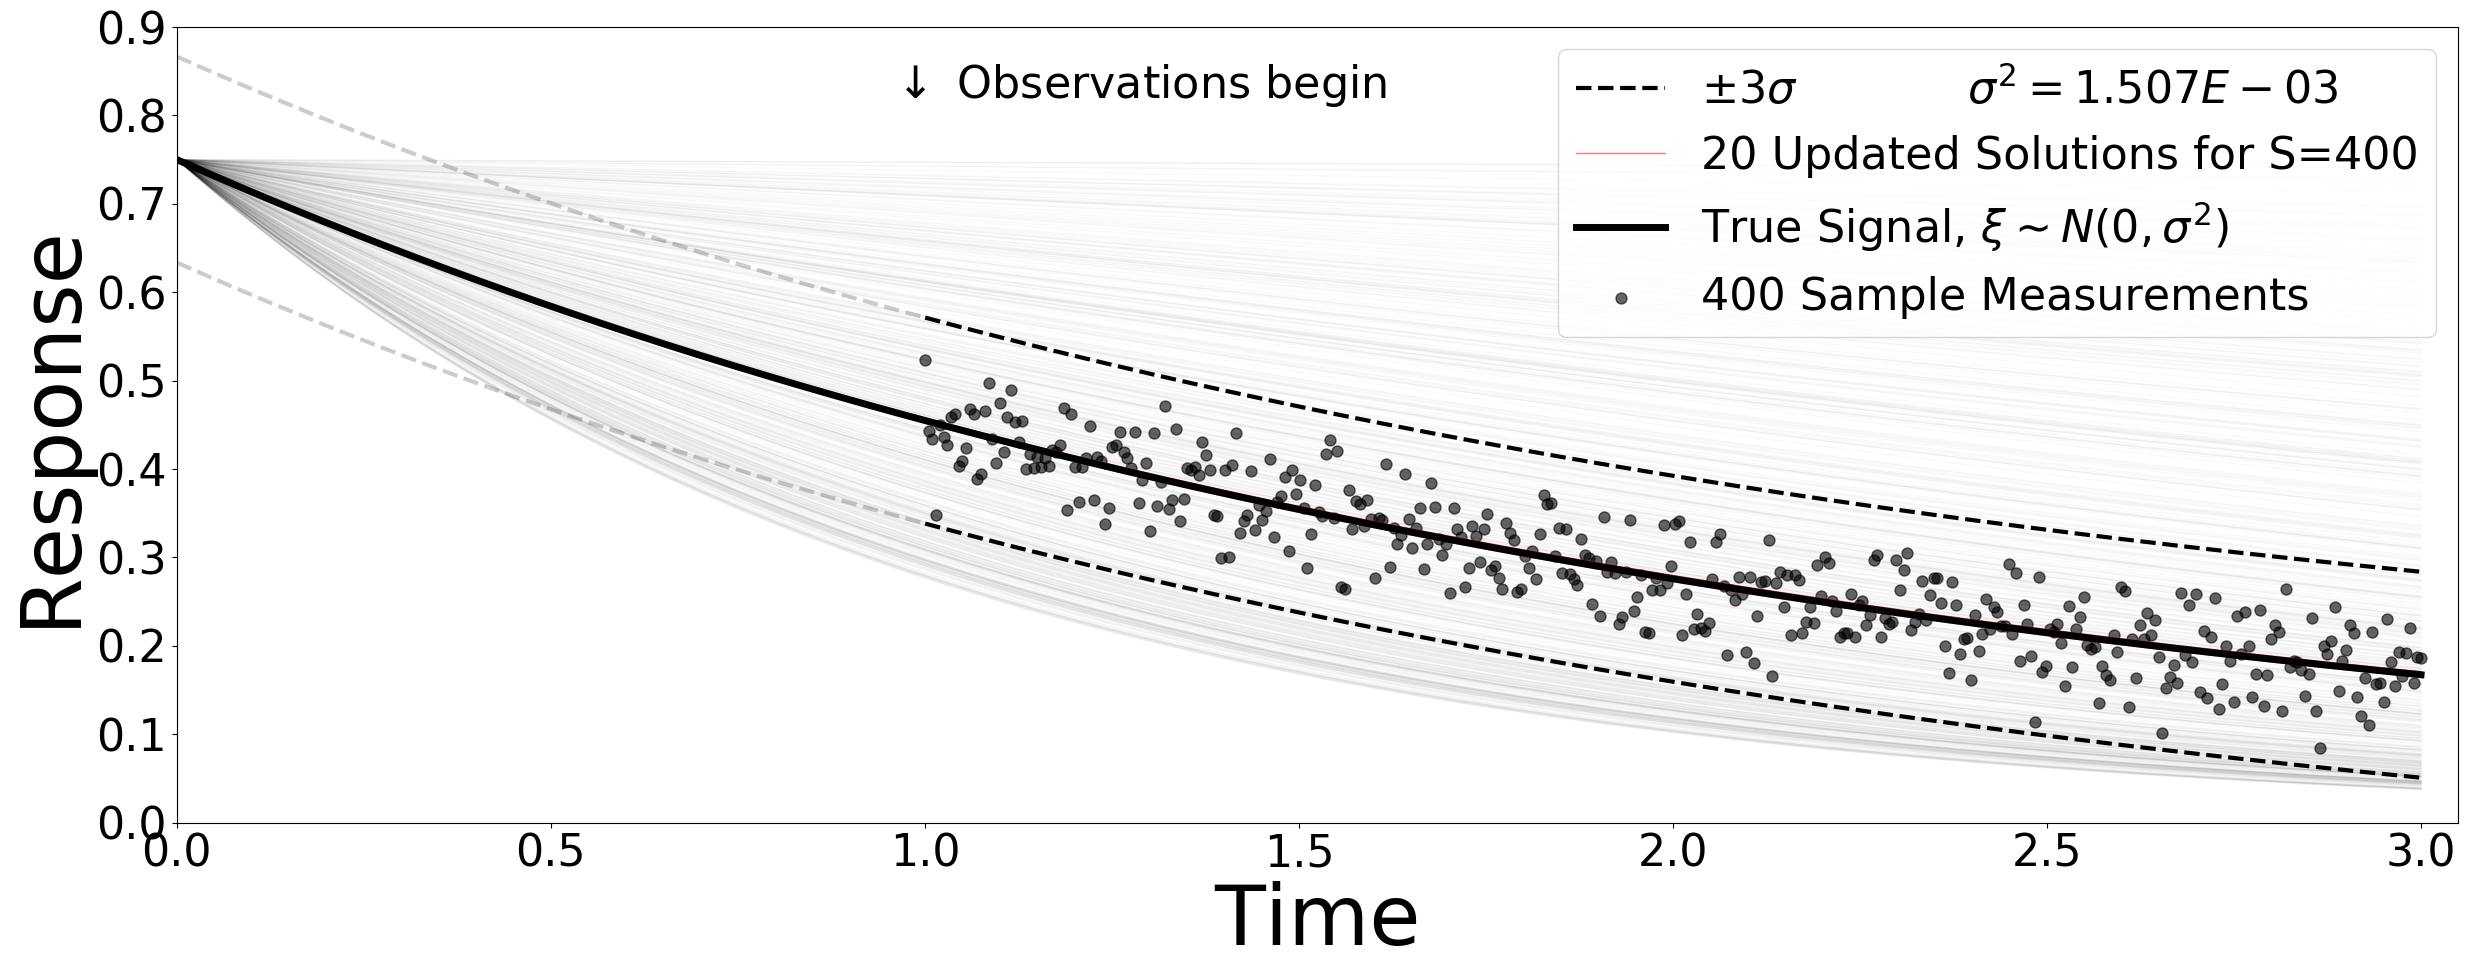
\includegraphics[width=\linewidth]{figures/ode/ode-alt_400_reference_solution.png}
  \caption{Gray lines are the initial parameter samples.
  The true signal (black) is well-recovered by the MUD estimates (red).
  (Top): First twenty measurements used to solve the original problem.
  (Middle): First twenty measurements used to solve the alternative problem.
  (Bottom): The entire value $\param_i$ ($1\leq i \leq N$), in the sampled parameter set.
  }
  \label{fig:ode-alt-reference}
\end{figure}

To quantify accuracy and stability of the MUD solutions, we solve the problem for the same choices of $S$ as the original problem (with the addition of $S=400$).
We show the resulting error plots for convergence in the right half of Figures~\ref{fig:ode-convergence-alt}, juxtaposed against the original experimental design with $100$Hz equipment.

\begin{figure}[htbp]
  \centering
  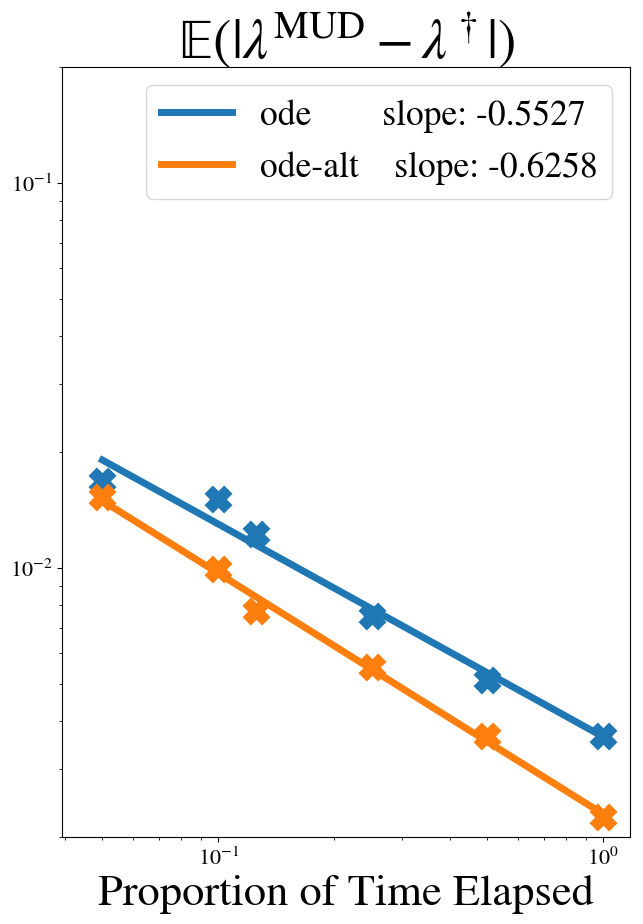
\includegraphics[width=0.475\linewidth]{figures/ode/ode_convergence_mud_obs_mean_comp.png}
  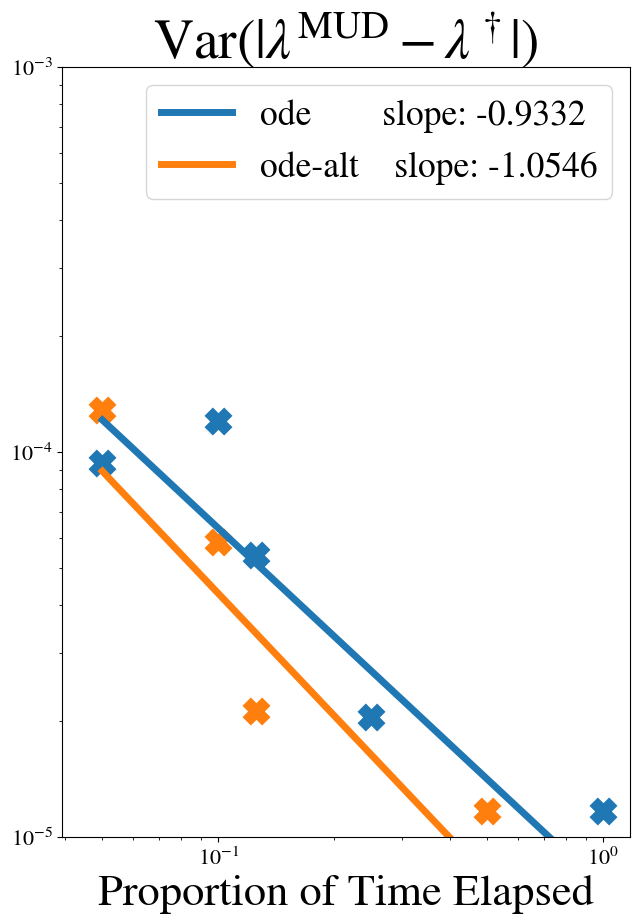
\includegraphics[width=0.425\linewidth]{figures/ode/ode_convergence_mud_obs_var_comp.png}

  \caption{Convergence of the MUD point given $N=1E3$ model evaluations for increasing numbers of observations for randomly placed sensors.
  Convergence rates are estimated using first-order linear regressions in $\text{log}_{10}$-space.
  $100$Hz equipment demonstrates a reduction of uncertainty and improvement in precision as $S$ increases towards $200$.
  We observe the same rates of convergence for the alternative equipment and note the (slightly) lower overall error for equal numbers of measurements ($S=200$ corresponding to $t\in (1,2)$ in this formulation).
  }
  \label{fig:ode-convergence-alt}
\end{figure}

The convergence rates are similar (shown in the legend of \ref{fig:ode-convergence}), and reduction in uncertainty is almost negligible at a given $S$.
However, we note that in the alternative setup, for an equal number of measurements, the time elapsed is half of that in the original due to the different equipment being used.
To this end, we estimate convergence rates with respect to the time elapsed in the experiment rather than number of measurements used, and notice that the alternative setup (orange) exhibits much lower error at a given point of time.
This implies that we can achieve similar results with a shorter observational window by using equipment that allows for faster observations.



%%%%%%%%%%%%%%%%%%%%%%%%%%%%%%%%%%%%%%%%%%%%%%%%%%%%%%%%%%%%%%%%%%%%
\FloatBarrier
%%%%%%%%%%%%%%%%%%%%%%%%%%%%%%%%%%%%%%%%%%%%%%%%%%%%%%%%%%%%%%%%%%%%

\subsection{Impact of Equipment Precision}
To achieve higher precision in the estimate of the MUD point, one can use more precise measurement equipment.
We expect that a method designed to address parameter estimation would see an improvement in accuracy  if the data is collected with more precise instruments.
Here we show that this is indeed the case for the time-series example introduced earlier by considering choices of $\tau = 0.1, 0.05, 0.01, \text{ and } 0.005$ for $\mathbb{P}( \abs{\xi} < \tau ) = 99\%$ to select our $\sigma$ in our normal additive noise model.
We sequentially incorporate $S=5, 10, 15, 20, 25, 50, 100, \text{ and } 200$ measurements and study the error in our estimate of $\paramref$.



\begin{figure}[htbp]
  \centering
  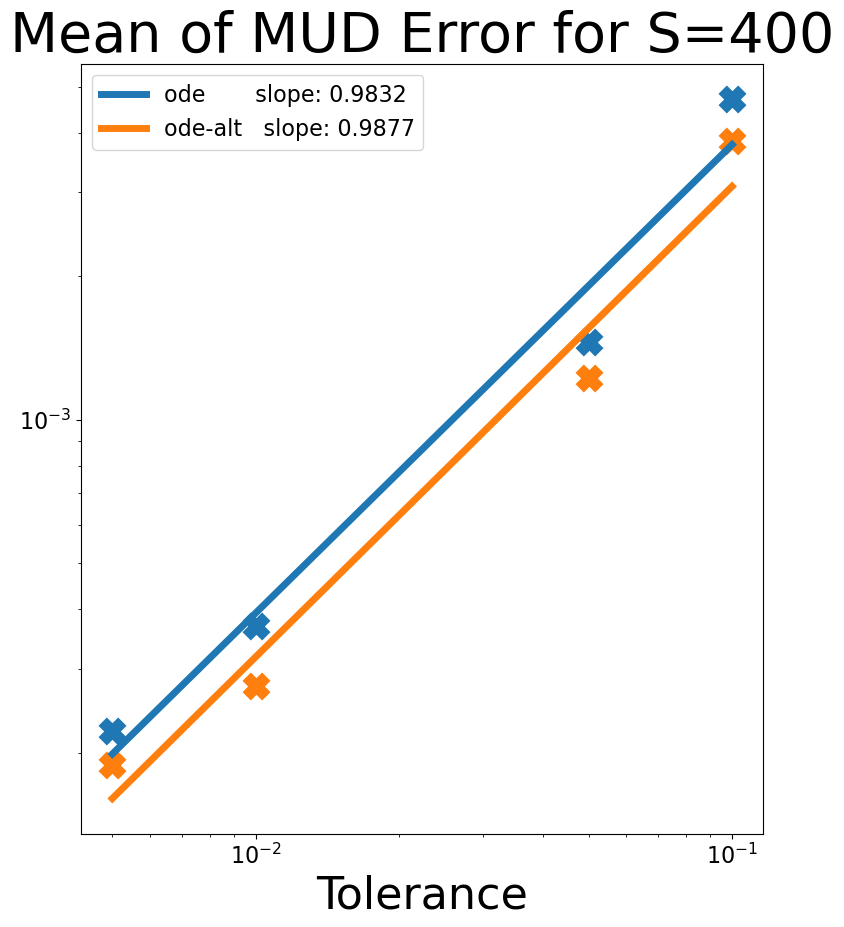
\includegraphics[width=0.475\linewidth]{figures/ode/ode_convergence_mud_std_mean.png}
  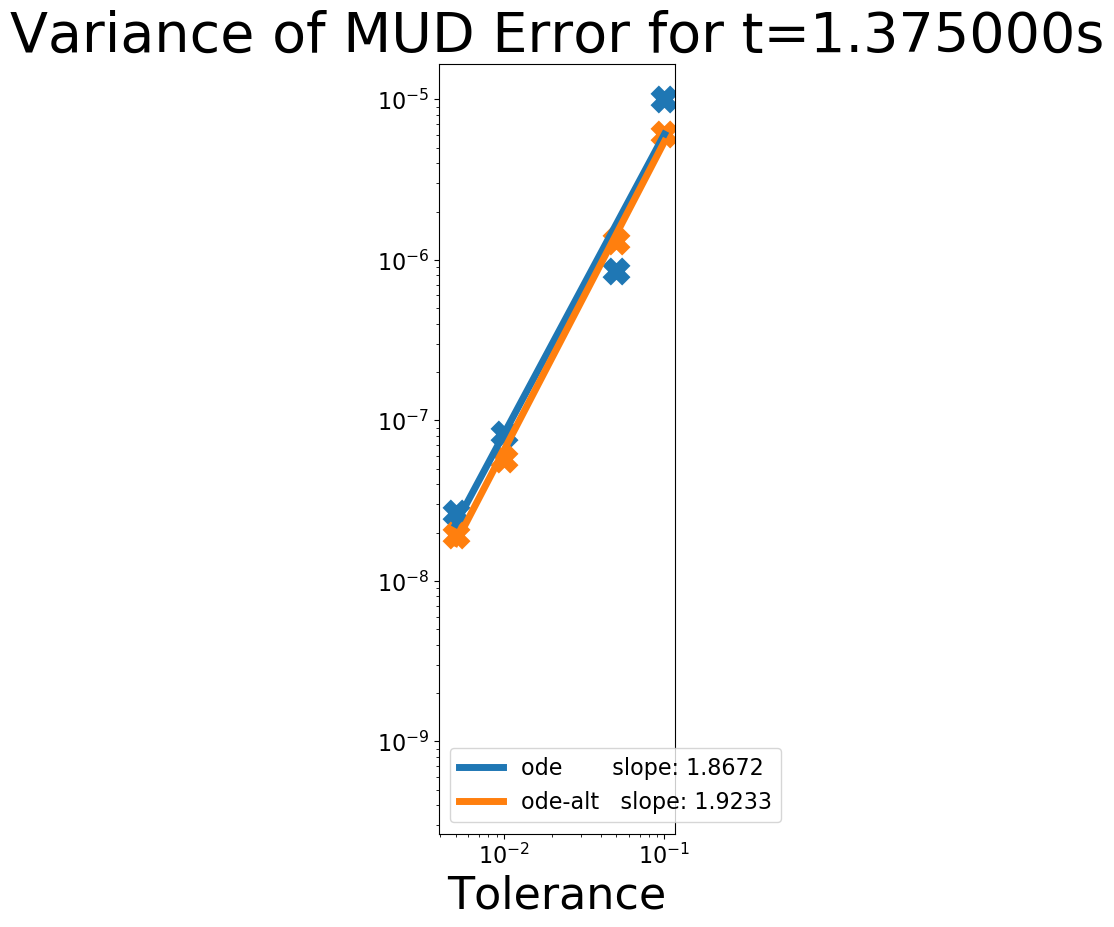
\includegraphics[width=0.425\linewidth]{figures/ode/ode_convergence_mud_std_var.png}

  \caption{Convergence of the MUD point given $N=1E3$ model evaluations incorporating measurements at a fixed point in time.
  As more precise measurements are incorporated, the accuracy and precision of the MUD solution improves.
  }
  \label{fig:ode-convergence-std}
\end{figure}

In Figure~\ref{fig:ode-convergence-std}, we study the absolute error's mean and variance as our measurement equipment gets more precise (lower tolerance), for both the $100$Hz (ode) and $200$Hz (ode-alt) variants of sensors we are simulating.
In the left half of the figure, we find that the convergence rates for the two designs are nearly identical but the equipment which records twice as many measurements has a persistent reduction in error.
The right half shows the convergence in variance of the absolute error, and the vertical displacement between the two designs is visually difficult to distinguish.
However, as evidenced in the legend annotations of Fig~\ref{fig:ode-convergence-std}, the alternative design (faster equipment) exhibits an increase in the rate of convergence from 1.87 to 1.92.

We have shown that the Data--Consistent approach to solving parameter identification problems manages to generalize to problems involving time-series data from a single Quantity of Interest.
We now turn our attention to an example where instead of temporal measurements, we incorporate spatial data to solve another 1-D parameter identification problem.
